% \RequirePackage{scrlfile}
% \makeatletter
% \AfterPackage{beamerbasemodes}{\beamer@amssymbfalse}
% \makeatother

\documentclass{beamer}

\usepackage{bookmark}
\usepackage{fix-cm}
\usepackage[ngerman]{babel} 
\usepackage[utf8]{inputenc}
\usepackage[T1]{fontenc}

\usepackage{tgschola}
% \usepackage{droid}
% \usepackage{bera}
% \usepackage[boldsans]{concmath}
\renewcommand{\ttdefault}{lmtt}
\usefonttheme{serif}

\usepackage{listings}
\lstset{language=C}
\lstset{showstringspaces=false}
\lstset{basicstyle=\ttfamily}
\lstset{commentstyle=\slshape}
\lstset{keywordstyle=\color{teal}}
\lstset{mathescape=true}

\usepackage{booktabs}

\usepackage{tikz}
\usetikzlibrary{arrows,matrix,decorations.pathreplacing,shapes}
\tikzset{>=stealth'}
\tikzset{decoration={brace,amplitude=8pt,mirror}}

\usepackage{graphicx}
\graphicspath{{./Debugger/}}

\usetheme[compress]{Dresden}
% \usetheme{Pittsburgh}
\usecolortheme{dove}
% \usecolortheme{seagull}
% this will eliminate warnings about font size substitution
% when using concrete roman
% \setbeamerfont{sidebar}{size=\tiny}

\setbeamertemplate{navigation symbols}{}
\setbeamertemplate{footline}[frame number]
\AtBeginPart{%
\frame{\partpage}%
\frame[allowframebreaks]{\frametitle{Inhalt}\tableofcontents}}


\title{UMach}
\subtitle{eine virtuelle Maschine}
\author{}
\institute{Georg-Simon-Ohm-Hochschule}
\date{}


%%%% When printing, put 4 pages on 1
% \usepackage{pgfpages}
% \pgfpagesuselayout{4 on 1}[a4paper,border shrink=2mm,landscape]

\begin{document}

\frame{\titlepage}


\begin{frame}{Überblick}
 \begin{enumerate}
  \item Projektbeschreibung
  \item Architektur
  \item Assembler
  \item Debugging
  \item Demos
 \end{enumerate} 
 UMach ist eine sehr lange Geschichte\ldots
\end{frame}



\part{Projektbeschreibung}
\section{Projektvorstellung}

Das IT-Projekt wurde während des SS 2012 und WS 2012/13 durchgeführt. Ziel
dieses Projektes war die Spezifikation und Implementieung einer virtuellen
Maschine namens UMach. Dazu gehören ein Assembler und ein Debugger für diese
Maschine. Der gewünschte Workflow bei der Fertigstellung des Projektes war der
folgende:

\begin{enumerate}
\item Der Benutzer schreibt eine Assembler-Datei. Diese enthält Anweisungen an
die UMach-Maschine wie die folgenden:
\begin{lstlisting}
SET  R2 0x1A
MULI R2 4
CP   R2 LO
SET  R1 0
SW   R1 R2
\end{lstlisting}
Wir nehmen an, die Datei heißt \glqq{}test.uasm\grqq{}.

\item Diese Datei wird in eine Bytecode-Datei assembliert mit dem folgenden
Befehl:
\begin{lstlisting}
./uasm -o test.umx test.uasm
\end{lstlisting}
Ergebnis ist eine Bytecode-Datei namens \glqq{}test.umx\grqq{}. Diese
Bytecode-Datei enthält UMach-Instruktionen in binärer Form. Die oben angegebenen
Instruktionen werden wie folgt assembliert:
\begin{lstlisting}
0x10 0x02 0x00 0x1A
0x3A 0x02 0x00 0x04
0x11 0x02 0x2B 0x00
0x10 0x01 0x00 0x00
0x15 0x01 0x02 0x00
\end{lstlisting}

\item Die Bytecode-Datei wird von der UMach-Maschine ausgeführt mit dem
folgenden Befehl:
\begin{lstlisting}
./umach test.umx
\end{lstlisting}
Alternativ kann man die Maschine in Debugg-Modus starten mit dem Befehl
\begin{lstlisting}
./umach -d test.umx
\end{lstlisting}
Alternativ steht ein getrennter Qt-Debugger zur Verfügung.
\end{enumerate}

Diesen Workflow betrachten wir als implementiert. Alle diese Schritte sind
möglich und liefern die gewünschten Ergebnisse. Das Projekt enthält auch eine
Reihe von fertiggeschriebenen Assembler-Programmen, die gleich getestet werden
können.


\subsection{Teilaufgaben}

Im Rahmen dieses Projektes wurden die folgenden Teilaufgaben übernommen und
gelöst.

\begin{enumerate}
\item Konzeptioneller Entwurf der virtuellen Maschine.
\item Spezifikation der virtuellen Maschine als PDF Dokument (Liviu Beraru).
\item Implementieung der Maschine in C99 für Linux (Liviu Beraru).
\item Assembler für die Maschine in C99 für Linux (Werner Linne).
\item Qt-Debugger (Simon Beer).
\item Demonstrationsprogramme in der UMach Assemblersprache \texttt{uasm} 
      (Willi Fink).
\item Anweisungen zur Verwendung der UMach virtuellen Maschine, als PDF
Dokument.
\end{enumerate}

Die späteren Abschnitte gehen auf die Lösungswege der einzelnen Teilaufgabe
ein. Jeder Abschnitt wurde vom zuständigen Gruppenmiglied geschrieben.


\subsection{Organisation}

Die Kommunikation unter den Gruppenmiglieder lief über Email, persönlichen
Gespräche, Telefonaten und TODO-Dateien. Für die Verwaltung aller \LaTeX{} und C
Dateien wurde das Versionsverwaltungssystem GIT verwendet. Für die zentralle
Verwaltung aller Dateien wurde ein GIT-Account auf Github eingerichtet und dort
ein Projekt angelegt. Das Projekt ist öffentlich zugänglich, Schreiberechte aber
haben nur die Gruppenmiglieder. Das Projekt kann unter der Adresse

\url{https://github.com/Malkavian/UMachVM}

nachgeschlagen werden. Dort können alle Dateien heruntergeladen werden.


\part{Architektur und Implementierung}
\section{Architektur}

\subsection{Maschinentyp}

\begin{frame}[fragile]{\insertsubsection}
 \begin{itemize}
  \item UMach ist eine registerbasierte RISC Maschine.\\
        
        Wenige Befehle (69) mit fester Länge.        
  \item Load/Store Speicherzugriff über Registerangabe.
\begin{lstlisting}
LW   R1 R2 # R1 $\gets$ mem(R2)
SW   R1 R2 # R1 $\to$ mem(R2)
\end{lstlisting}
  \item Port I/O
\begin{lstlisting}
IN  R17 R18 R19
OUT R1  R2  R3
\end{lstlisting}
  \item Keine Pipeline
  \item Big endian
 \end{itemize}
\end{frame}


\subsection{Register}

\begin{frame}{\insertsubsection}
 Die UMach Maschine hat 32 Allzweckregister
 und 13 Spezialregister.
 
 Jedes Register ist genau 32 Bit lang.
 
 Die Register werden intern durch Nummern identifiziert:
 Register Nummer 0, Nummer 1, Nummer 2\ldots{} Nummer 44.
\end{frame}


\subsubsection{Allzweckregister}

\begin{frame}{\insertsubsubsection}
 Die Register mit Nummern 1 bis 32 können frei verwendet werden.
 Sie werden von der Maschine ohne explizite Anweisung nicht geändert, außer
 dass sie beim Start der Maschine mit dem Wert Null belegt werden.

 Die Allzweckregister haben die Namen $R1$, $R2$, \ldots{} $R32$.
 
 Register mit den Namen $R0$ und $R33$ gibt es nicht.
\end{frame}



\subsubsection{Spezialregister}

\begin{frame}{\insertsubsubsection}
 Dienen der Steuerung der Maschine und haben besondere Aufgaben. Sie werden von
 der Maschine verändert.
 
 Die meisten sind schreibgeschützt.
\end{frame}

\begin{frame}{\insertsubsubsection{} - Liste}
 \begin{tabular}{lcl}
Name  & Nummer & Beschreibung \\\toprule
PC    & 33     & Program Counter   \\ 
DS    & 34     & Data Section (begin)   \\ 
HS    & 35     & Heap Section (first byte)   \\ 
HE    & 36     & Heap Section (last byte)   \\ 
SP    & 37     & Stack Pointer   \\ 
FP    & 38     & Frame Pointer  \\ 
IR    & 39     & Instruction Register   \\ 
STAT  & 40     & Status Register   \\ 
ERR   & 41     & Error Register   \\ 
HI    & 42     & Higher 32 Bits (Division, Multiplik.)   \\ 
LO    & 43     & Lower 32 Bits (Division, Multiplik.)   \\ 
CMPR  & 44     & Ergebniss von CMP   \\ 
ZERO  & 0      & Immer konstant Null   \\\bottomrule
 \end{tabular}
\end{frame}




\subsection{Befehle}

\begin{frame}{\insertsubsection}
 Ein Befehl ist immer 32 Bits lang (4 Byte), auch wenn er keine Argumente nimmt
 (RISC Architektur).
 Erstes Byte ist der Befehl, die anderen 3 Bytes sind eventuelle Argumente.
 \begin{center}
   
\begin{tikzpicture}

\tikzstyle{lab}=[midway,yshift=-10pt,align=center,anchor=north]

  \matrix (m) 
 [matrix of nodes,
  nodes={draw,text height=2ex,text depth=0.25ex,
  minimum width=5em,font=\ttfamily}]
 {
    0x30 & 0x03 & 0x01 & 0x02 \\
 };
 
 \draw[decorate] (m-1-1.south west) -- (m-1-1.south east) 
  node [lab] {Befehl};
 \draw[decorate] (m-1-2.south west) -- (m-1-4.south east) 
  node [lab] {Argumente};
\end{tikzpicture}

 \end{center} 
\end{frame}



\subsection{Befehlsformate}

\begin{frame}{\insertsubsection}
 Wie MMIX von Knuth, hat UMach mehrere Befehlsformate, d.h. mehrere Arten, wie
 man die Argumente einteilen und interpretieren kann.
 
 Manche Befehle erwarten Registernummern, andere direkte nummerische Angaben
 verschiedener Längen, andere eine Mischung davon, andere keine Argumente.
\end{frame}


\begin{frame}{\insertsubsection}
 \begin{center}
  \begin{tabular}{l||c|c|c}
    \toprule
    Format & zweites Byte  & drittes Byte  & viertes Byte \\\toprule
    000 & \multicolumn{3}{c}{nicht verwendet}           \\\midrule
    NNN & \multicolumn{3}{c}{3 Bytes Zahl}              \\\midrule
    R00 & $R_{1}$ & \multicolumn{2}{c}{nicht verwendet} \\\midrule
    RNN & $R_{1}$ & \multicolumn{2}{c}{2 Bytes Zahl}    \\\midrule
    RR0 & $R_{1}$ & $R_{2}$ &  nicht verwendet           \\\midrule
    RRN & $R_{1}$ & $R_{2}$ &  1 Byte Zahl               \\\midrule
    RRR & $R_{1}$ & $R_{2}$ & $R_{3}$                    \\\bottomrule
  \end{tabular}
\end{center}
($R_{1}$, $R_{2}$, $R_{3}$: erste, zweite, dritte Registernummer)

Alle Zahlenangaben: big endian.
\end{frame}



\begin{frame}{\insertsubsection{} - Beispiel RRR}
 \texttt{ADD}: drei Registernummern.
 \begin{center}
   
\begin{tikzpicture} [font=\ttfamily]

\tikzstyle{lab}=[midway,yshift=-10pt,align=center,anchor=north]

  \matrix (m) 
 [matrix of nodes,
  nodes={draw,text height=2ex,text depth=0.25ex,
  minimum width=5em}]
 {
    0x30 & 0x03 & 0x01 & 0x02 \\
 };
 
 \draw[decorate] (m-1-1.south west) -- (m-1-1.south east) node [lab] {ADD};
 \draw[decorate] (m-1-2.south west) -- (m-1-2.south east) node [lab] {R3};
 \draw[decorate] (m-1-3.south west) -- (m-1-3.south east) node [lab] {R1};
 \draw[decorate] (m-1-4.south west) -- (m-1-4.south east) node [lab] {R2};
\end{tikzpicture}

 \end{center}
\end{frame}

\begin{frame}{\insertsubsection{} - Beispiel RNN}
 \texttt{DIVI}: eine Registernummer und eine 2-Byte Zahl.
 \begin{center}
   
\begin{tikzpicture} [font=\ttfamily]

\tikzstyle{lab}=[midway,yshift=-10pt,align=center,anchor=north]

  \matrix (m) 
 [matrix of nodes,
  nodes={draw,text height=2ex,text depth=0.25ex,
  minimum width=5em}]
 {
    0x3D & 0x03 & 0x01 & 0x02 \\
 };
 
 \draw[decorate] (m-1-1.south west) -- (m-1-1.south east) node [lab] {DIVI};
 \draw[decorate] (m-1-2.south west) -- (m-1-2.south east) node [lab] {R3};
 \draw[decorate] (m-1-3.south west) -- (m-1-4.south east) node [lab] {0x0102};
\end{tikzpicture}

 \end{center}
\end{frame}

\begin{frame}{\insertsubsection{} - Beispiel NNN}
 \texttt{JMP}: ein 3-Byte Offset (vorzeichenbehaftet).
 \begin{center}
   
\begin{tikzpicture} [font=\ttfamily]

\tikzstyle{lab}=[midway,yshift=-10pt,align=center,anchor=north]

  \matrix (m) 
 [matrix of nodes,
  nodes={draw,text height=2ex,text depth=0.25ex,
  minimum width=5em}]
 {
    0x88 & 0xFF & 0xFF & 0xFD \\
 };
 
 \draw[decorate] (m-1-1.south west) -- (m-1-1.south east) node [lab] {JMP};
 \draw[decorate] (m-1-2.south west) -- (m-1-4.south east) node [lab] {-3};
\end{tikzpicture}

 \end{center}
\end{frame}

\subsection{Befehlsmenge}

\begin{frame}{\insertsubsection}
\begin{enumerate}
  \item Kontrollinstruktionen: \texttt{NOP}, \texttt{EOP}
  \item Lade- und Speicherbefehle: 
        \texttt{SET}, \texttt{LW}, \texttt{SB}, \texttt{PUSH}
  \item Arithmetische Instruktionen:
        \texttt{ADD}, \texttt{SUB}, \texttt{INC}
  \item Logische Instruktionen:
        \texttt{AND}, \texttt{XOR}, \texttt{SHL}, \texttt{ROTL}
  \item Vergleichsinstruktionen:
        \texttt{CMP}, \texttt{CMPI}
  \item Sprunginstruktionen:
        \texttt{JMP}, \texttt{BE}, \texttt{BL}
  \item Unterprogramminstruktionen:
        \texttt{CALL}, \texttt{RET}, \texttt{GO}
  \item Systeminstruktionen:
        \texttt{INT}
  \item I/O Instruktionen:
        \texttt{IN}, \texttt{OUT}
\end{enumerate}
Insgesamt 69 Befehle.
\end{frame}



\subsection{Speichermodell}

\begin{frame}{\insertsubsection}
 Der Speicher der UMach Maschine enthält hauptsächlich
 \begin{itemize}
  \item Programmcode
  \item Programmdaten
  \item Freier Speicher
 \end{itemize}
  Kein Memory Mapped I/O.
  
  Gesamte Speichergröße ist nach dem Start der Maschine fest.
\end{frame}


\begin{frame}{Segmente}
 Der Speicher wird in Segmenten eingeteilt.
 \begin{enumerate}
  \item Interrupttabelle
  \item Programmcode (Code-Segment)
  \item Programmdaten (Daten-Segment)
  \item Heap (Freispeicher)
  \item Stack (Lokaler Speicher)
 \end{enumerate}
 Der Code- und Daten-Segment werden aus der Programmdatei geladen. 
 Der Rest ist dynamisch und kann durch Register (\texttt{HE}, \texttt{SP})
 oder Befehle (\texttt{PUSH}, \texttt{POP}) manipuliert werden.
\end{frame}


\begin{frame}[fragile]{Heap und Stack Manipulieren}
 \begin{lstlisting}
  ADDI HE HE 128
  # ...
  SUBI HE HE 128
 \end{lstlisting}
 Speicher auf dem Heap reservieren erfolgt dadurch, dass der Inhalt des
 Registers \texttt{HE} (Heap End) hochgezählt wird. Speicher freigeben durch
 runterzählen.
 
 \begin{lstlisting}
  SUBI SP SP 32
  # ...
  ADDI SP SP 32
 \end{lstlisting}
 Lokaler Speicher wird durch Veränderung des Registers \texttt{SP} (Stack
 Pointer) erreicht.
\end{frame}


\begin{frame}{Speicher-Layout}
 \begin{center}
   
\begin{tikzpicture}
\tikzset{
  mmatrix/.style={
    matrix of nodes,
    nodes={
      draw,
      minimum height=8ex,
      text depth=0ex,
      align=center,
      anchor=center,
      font=\small
    }
  }
};

\tikzstyle{lab}=[yshift=-2ex,anchor=center]

 \matrix (m) [mmatrix]
 {
    |[text width=1.7cm]|Interrupt\-tabelle & 
    Programm & Daten & Heap & frei & Stack \\
 };

  \draw[thick] (m-1-1.north west) -- ++(0,-2) node[lab] {0};
  \draw[thick] (m-1-1.north east) -- ++(0,-2) node[lab] {256};
  \draw[thick] (m-1-2.north east) -- ++(0,-2) node[lab] {DS};
  \draw[thick] (m-1-3.north east) -- ++(0,-2) node[lab] {HS};
  \draw[thick,dashed] (m-1-4.north east) -- ++(0,-2) node[lab] {HE};
  \draw[thick,dashed] (m-1-5.north east) -- ++(0,-2) node[lab] {SP};
  \draw[thick] (m-1-6.north east) -- ++(0,-2) node[lab] {max};
\end{tikzpicture}

 \end{center}
 Segmentation Fault: schreiben in Code-Segment.
 
 Stack Overflow: Befehl \texttt{PUSH} führt zum Überlappen der Register
\texttt{SP} und \texttt{HE}.
\end{frame}



\subsection{I/O}

\begin{frame}{Port I/O}
 Die UMach Maschine verwendet Port I/O, d.h. sie hat Befehle zum Ausgeben und
 Einlesen von Daten. Es werden Ports verwendet: durchnummerierte Ausgänge und
 Eingänge.
\end{frame}

\begin{frame}{Ports}
 Es gibt 8 Ausgabeports und 8 Eingabeports, die jeweils von 0 bis 7
 durchnummeriert sind.
 
 Ausgabeport 0: \texttt{stdout}.
 
 Eingabeport 0: \texttt{stdin}.
\end{frame}


\begin{frame}{Transfer}
 Der Datentransfer findet direkt zwischen Speicher und I/O-Ports statt.
 Der Transfer blockiert die Maschine solange der Transfer noch nicht fertig ist.
 
 Die I/O-Befehle haben das Format RRR (drei Registernummern).
\end{frame}


\begin{frame}{Ausgabe}
 Die Ausgabe erfolgt durch verwendung des Befehls \texttt{OUT}
 \begin{center}
   
\begin{tikzpicture}

\tikzstyle{lab}=[midway,yshift=-10pt,align=center,anchor=north,font=\small]

  \matrix (m) 
 [matrix of nodes,
  nodes={draw,
         text height=2ex,text depth=0.25ex,
         minimum width=5em,
         font=\ttfamily}]
 {
    OUT & R1 & R2 & ZERO \\
 };
 
 \draw[decorate] (m-1-1.south west) -- (m-1-1.south east) node [lab] {Ausgabe};
 \draw[decorate] (m-1-2.south west) -- (m-1-2.south east) 
                 node [lab] {Adresse\\ im Speicher};
 \draw[decorate] (m-1-3.south west) -- (m-1-3.south east) 
                 node [lab] {Anzahl\\ bytes};
 \draw[decorate] (m-1-4.south west) -- (m-1-4.south east) 
                 node [lab] {Portnummer};
 
\end{tikzpicture}

 \end{center}
\end{frame}


\begin{frame}{Eingabe}
 Die Eingabe erfolgt durch verwendung des Befehls \texttt{IN}
 \begin{center}
   
\begin{tikzpicture}

\tikzstyle{lab}=[midway,yshift=-10pt,align=center,anchor=north,font=\small]

  \matrix (m) 
 [matrix of nodes,
  nodes={draw,
         text height=2ex,text depth=0.25ex,
         minimum width=5em,
         font=\ttfamily}]
 {
    IN & HS & R2 & ZERO \\
 };
 
 \draw[decorate] (m-1-1.south west) -- (m-1-1.south east) node [lab] {Eingabe};
 \draw[decorate] (m-1-2.south west) -- (m-1-2.south east) 
                 node [lab] {Zieladresse\\ im Speicher};
 \draw[decorate] (m-1-3.south west) -- (m-1-3.south east) 
                 node [lab] {Anzahl\\ bytes};
 \draw[decorate] (m-1-4.south west) -- (m-1-4.south east) 
                 node [lab] {Portnummer};
 
\end{tikzpicture}

 \end{center}
\end{frame}


\subsection{Interrupts}

\begin{frame}{\insertsubsection}
 Unterbrechungen im normalen Programmfluss, die mit einer Interruptnummer
 versehen sind und die abgefangen werden können. 
 Analog zu \glqq exceptions\grqq{} in Java/C++.
 
 Abfangen heißt, dass eine Subroutine mit der Interruptnummer verbunden wird.
 
 Ist ein Interrupt nicht mit einer Subroutine verbunden, so stoppt die Maschine
 wenn der Interrupt passiert.
\end{frame}



\begin{frame}{Arten von Interrupts}
 \begin{enumerate}
  \item Hardware-Interrupts: wenn etwas schief mit einem Befehl geht:
        Division durch Null, Stack Overflow, falsche Befehlsnummer, ungültige
        Speicheraddresse, schreiben in das Codesegment, etc.
  \item Software-Interrupts: werden vom Programmierer durch den Befehl 
        \texttt{INT} angestoßen.
 \end{enumerate}
\end{frame}


\begin{frame}{Interrupttabelle}
 Die Interrupttabelle startet an der Addresse Null und besteht aus 64 Einträgen,
 jeweils 32 Bit groß (=256 Bytes).
 
 Jeder der $64$ Einträge entspricht einer Interruptnummer.
 
 Interrupt 26 $\to$ Adresse $26 \cdot 4 = 104$.
 
 An jedem Index steht entweder Null oder die Addresse einer Subroutine
 (Interrupt Handler). Diese wird ausgeführt, wenn der entsprechende Interrupt
 generiert wird.
 
 Adresse des Interrupt Handlers ist Null $\mapsto$ Maschine ausschalten.
\end{frame}



\begin{frame}{Wie läuft ein Interrupt ab}
 \begin{center}
  \begin{tikzpicture} [->,node distance=1.8cm,auto]

\tikzset{every label/.style={font=\scriptsize,red!80!black}}
\tikzstyle{start}=[draw=blue!20!black,circle]
\tikzstyle{block}=[draw]
\tikzstyle{end}  =[draw=green!60!black,rounded corners,double]
\tikzstyle{err}  =[draw=red!60!black,rounded corners,double]
\tikzstyle{ask}  =[draw,diamond,align=center,text badly centered,inner sep=0pt,
                   text width=4em,aspect=2]
\tikzstyle{away} =[node distance=4cm]

 
 
 \node[start,label=below:{segfault}]
                              (A) {\texttt{INT} $x$};
 \node[ask,right of=A,away]   (B) {$x \geq 0 \;\land\; x \leq 63$?};
 \node[block,right of=B,away] (C) {$x \gets 0$};
 \node[block,below of=B]      (D) {$y \gets$ interrupt\_table[$x$]};
 \node[ask,below of=D]        (E) {$y = 0$?};
 \node[err,right of=E,away]   (F) {stop Umach};
 \node[end,below of=E]        (G) {\texttt{PUSH PC}; \texttt{GOTO} $y$};

 \draw (A) --                  (B);
 \draw (B) -- node {nein}      (C);
 \draw (B) -- node {ja}        (D);
 \draw[rounded corners] (C) |- (D);
 \draw (D) --                  (E);
 \draw (E) -- node {ja}        (F);
 \draw (E) -- node {nein}      (G);
\end{tikzpicture}




 \end{center}
\end{frame}



\section{Implementierung}

\subsection{Programmablauf}

\begin{frame}[fragile]{\insertsubsection}
 Die Maschine hat grundsätzlich zwei Schritte, die sie immer wieder wiederholt: 
 fetch und execute. 
 \begin{lstlisting}
void core_run_program(void)
{
    while (running) {
        core_fetch();
        core_execute();
    }
}
 \end{lstlisting}
\end{frame}


\begin{frame}[fragile]{Fetch}
 Fetch: die nächste Instruktion aus dem Speicher holen.
\begin{lstlisting}
void core_fetch(void)
{
    if (! running) { return; }
    mem_read               // read from mem
    ( instruction,         // whereto
      registers[PC].value, // wherefrom
      4                    // how much
    );
}
\end{lstlisting}
Lese 4 Bytes aus dem Speicher ab der Adresse \texttt{PC} in den
Puffer \texttt{instruction}.

Nach \texttt{fetch} steht der neue Befehl im globalen Array
\texttt{instruction[4]}. (big endian)
\end{frame}



\begin{frame}[fragile]{Execute}
 Befehl ausführen und \texttt{PC} inkrementieren.
\begin{lstlisting}
struct command *cmd = 
       command_by_opcode(instruction[0]);
if   (cmd != NULL) 
     { cmd->opfunc();              } 
else { interrupt(INT_INVALID_CMD); }
registers[PC].value += 4;
\end{lstlisting}

Es wird nach einem Funktionszeiger gesucht, der dem Befehlscode entspricht
(die Funktion implementiert den Befehl).
Fall vorhanden, ausführen. Falls nicht, Interrupt generieren.

(Der Funktionszeiger ist in einer Struktur \texttt{command} gepackt.)
\end{frame}


\subsection{Sprungtabellen}

\begin{frame}{\insertsubsection}
 Wie wird schnell nach einem Funktionszeiger gesucht?
 
 Mit Sprungtabellen: ein Array von Funktionszeigern in Strukturen gepackt, wo
 jede Struktur genau an dem Index steht, der gleich dem entsprechenden
 Befehlscode ist.
 
 Suchaufwand $O(1)$. Schneller geht's nicht.
\end{frame}


\begin{frame}[fragile]{\insertsubsection{} -- Auszug}
\begin{lstlisting}
struct command opmap[OPMAX] = {
    [0x00] = {0x00, "NOP", core_nop ,NUL},
    [0x04] = {0x04, "EOP", core_eop ,NUL},
    [0x10] = {0x10, "SET", core_set ,RNN},
    ....
    [0x90] = {0x90, "GO" , core_go  ,R00},
    [0x91] = {0x91, "CALL, core_call,NNN},
    [0x92] = {0x92, "RET", core_ret ,NUL},
    [0xA0] = {0xA0, "INT", core_int ,NNN},
    [0xB0] = {0xB0, "IN" , core_in  ,RRR},
    [0xB8] = {0xB8, "OUT", core_out ,RRR}
};
\end{lstlisting}
(C99 Magie.)
\end{frame}

\begin{frame}[fragile]{Suchen in der Sprungtabelle}
 Wie findet mal die Funktion, die einem Befehlscode entspricht?
\begin{lstlisting}
struct command* command_by_opcode
(int opcode)
{  
    if (opmap[opcode].opname) {
        return & opmap[opcode];
    } else {
        return NULL;
    }
}
\end{lstlisting}
\end{frame}


\begin{frame}[fragile]{Ein Beispiel: \texttt{ADD}-Befehl}
Eintrag in der Sprungtabelle:
\begin{lstlisting}
[0x30] = {0x30, "ADD", core_add, RRR}
\end{lstlisting}

Der Befehl \texttt{ADD} hat die Befehlsnummer \texttt{0x30} und die Funktion
\texttt{core\_add} steht am Index \texttt{0x30} in der Sprungtabelle.
\end{frame}


\begin{frame}[fragile]{\texttt{ADD} -- Implementierung}
\begin{lstlisting}
int core_add(void) {
    int32_t a = 0; 
    int32_t b = 0;

    read_register  (instruction[2], &a   );
    read_register  (instruction[3], &b   );
    write_register (instruction[1], a + b);       
    return 0;
}
\end{lstlisting}
(Veränderte Version, Error Checks gelöscht).
\end{frame}





\part{Assembler}
%%%%%%%%%%%%%%%%%%%%
%%  (C) by init0  %%
%%%%%%%%%%%%%%%%%%%%

\section{Zielsetzung}

\subsection{Aufgabe des Assemblers}

\begin{frame}{\insertsubsection}
    Der Assembler übersetzt Quelltext in UMach Bytecode
    und erstellt Debuginformationen.
\end{frame}


\subsection{Erwünschte Eigenschaften}

\begin{frame}{\insertsubsection}
    \begin{itemize}
        \item ``Angenehme'' Syntax
        \item Performance
        \item Aussagekräftige Fehlermeldungen
        \item Nützliche Debuginformationen
    \end{itemize}
\end{frame}

\section{Bedienung \& Syntax}

\subsection{Bedienung}

\begin{frame}{\insertsubsection}
    Der Assembler ``\texttt{uasm}'' wird über eine Shell aufgerufen. \\~\\
    Aufrufsyntax: \texttt{uasm [-o outfile] [-g] [-w] file(s)}
\end{frame}

\subsection{Assembler Syntax Beispiel}

\begin{frame}[fragile]{\insertsubsection}
\begin{verbatim}
SET R1 hello
myloop:  #useful comment
    CALL println
    DEC R2
    CMP R2 ZERO
BNE myloop
#lines containing only a comment or nil are ignored
SET R1 9001
EOP
.data  #begin of data definitions
.string hello  "Hello World!"
.int    answer 42
.int    drink  0xCAFE
\end{verbatim}
\end{frame}

\subsection{Assembler Syntax Regeln}

\begin{frame}[fragile]{\insertsubsection}
    \begin{itemize}
        \item Beliebig viele \verb#`\t'# und \verb*#` '# vor und nach Tokens
        \item Nur Symbolbezeichner sind case-sensitiv
        \item Symbolbezeichner sind keine gültigen Zahlwerte
        \item Symbolbezeichner bestehen aus genau einem Wort
    \end{itemize}
\end{frame}

\begin{frame}[fragile]{\insertsubsection}
    \begin{itemize}
        \item Definition einer Sprungmarke endet mit \verb#`:'#
        \item Sprungmarken stehen in einer eigenen Zeile
        \item Für alle Dateien gilt der gleiche Namensraum
        \item Ab \verb|`#'| beginnt ein Kommentar bis einschl. \verb#`\n'#
    \end{itemize}
\end{frame}

\section{Implementierung}

\begin{frame}[fragile]{\insertsection}
    \begin{itemize}
        \item 2-pass Assembler, geschrieben in C99
        \item Abhängigkeiten: \texttt{glibc} und \texttt{glib}
        \item ca. 1500 LOC
    \end{itemize}
\end{frame}

\subsection{Datenstrukturen}

\begin{frame}{\insertsection}{\insertsubsection}
    Drei Hashtabellen für
    \begin{enumerate}
        \item Befehle \textit{(statisch)}
        \item Register \textit{(statisch)}
        \item Symbole \textit{(dynamisch)}
    \end{enumerate}
    Eine verkettete Liste für den Inhalt von Daten
\end{frame}

\subsection{Commands}

\begin{frame}[fragile]{\insertsubsection}
\begin{lstlisting}
typedef enum {
    CMDFMT_NUL, CMDFMT_NNN, CMDFMT_R00,
    CMDFMT_RNN, CMDFMT_RR0, CMDFMT_RRN,
    CMDFMT_RRR
} cmdformat_t;

typedef struct {
    uint8_t     opcode;
    char       *opname;
    cmdformat_t format;
    char        has_label;
} command_t;
\end{lstlisting}
\end{frame}

\subsection{Register}

\begin{frame}[fragile]{\insertsubsection}
\begin{lstlisting}
typedef struct {
    uint8_t regcode;
    char   *regname;
} register_t;
\end{lstlisting}
\end{frame}

\subsection{Symbole}

\begin{frame}[fragile]{\insertsubsection}
\begin{lstlisting}
typedef enum {
    SYMTYPE_JUMP,
    SYMTYPE_DATA
} symbol_type_t;

typedef struct {
    char         *sym_name;
    symbol_type_t sym_type;
    uint32_t      sym_addr;
} symbol_t;
\end{lstlisting}
\end{frame}

\subsection{Variablen}

\begin{frame}[fragile]{\insertsubsection}
\begin{lstlisting}
typedef struct {
    char *label;
    char *value;
} string_data_t;

typedef struct {
    char   *label;
    int32_t value;
} int_data_t;
\end{lstlisting}
\end{frame}

\begin{frame}[fragile]{\insertsubsection}
\begin{lstlisting}
typedef enum {
    DATATYPE_INT, DATATYPE_STRING
} data_type_t;

typedef struct {
    data_type_t type;
    union {
        string_data_t string_data;
        int_data_t    int_data;
    };
} data_t;
\end{lstlisting}
\end{frame}

\subsection{Assembler Pass 1}

\begin{frame}{\insertsection}{\insertsubsection}
    ``Predict''
    \begin{itemize}
        \item Findet Sprungmarken und berechnet deren Adresse
        \item Berechnet die Codegröße
        \item Speichert Werte von Daten
        \item Berechnet Adressen von Daten
    \end{itemize}
\end{frame}

\subsection{Assembler Pass 2}

\begin{frame}{\insertsection}{\insertsubsection}
    ``Execute''
    \begin{itemize}
        \item Generiert UMach Bytecode
        \item Generiert Debuginformationen
        \item Speichert Werte von Daten in das Outputfile
    \end{itemize}
\end{frame}

\section{Performance}

\begin{frame}[fragile]{\insertsection}
    $Durchsatz \approx 1.4 \times 10^6 \frac{Zeilen}{Sekunde}$
    (AMD Athlon II X2 250, 3 GHz) \\~\\
    Speicherbedarf wächst linear mit der Anzahl der Symbolen \\~\\
    Auflösung von Symbolen meist in $\mathcal{O}(1)$ \\~\\
    Keine linearen Suchen; Programmlaufzeit in $\mathcal{O}(n)$
\end{frame}

\section{Fehlerdiagnose}

\begin{frame}{\insertsection}
    Der \texttt{uasm} Assembler informiert den Benutzer u.a. über folgende
    Fehler im Quelltext:
    \begin{itemize}
        \item Unbekannte Befehle
        \item Ungültige Argumente zu einem Befehl
        \item Unbekannte Symbole (Sprungmarken und Variablen)
        \item Unbekannte Register
        \item Ungültige Deklaration einer Variable
        \item Re-Definition einer Sprungmarke
        \item etc\ldots{}
    \end{itemize}
\end{frame}

\begin{frame}[fragile]{\insertsection}
    Zusätzlich zur Art des Fehlers wird Name \& Zeilennummer der Quelltextdatei
    in welcher der Fehler gefunden wurde ausgegeben.\\~\\
    Beispiele:
\begin{verbatim}
echo.uasm, line 1: No such command: <FOO>
echo.uasm, line 2: Command <CMP> expects RR0: REG,REG
echo.uasm, line 3: Unset label <getinput>
echo.uasm, line 4: Not a register: <R77>
echo.uasm, line 6: Label <get_input> already exists
echo.uasm, line 8: No content for .int provided
\end{verbatim}
\end{frame}

\section{Debuginformationen}

\begin{frame}{\insertsection}
    Wird das generieren von Debuginformationen per ``\texttt{\$uasm~-g}~\ldots''
    aktiviert, werden folgende Dateien erstellt:
    \begin{itemize}
        \item \texttt{u.out.fmap}
        \item \texttt{u.out.sym}
        \item \texttt{u.out.debug}
    \end{itemize}
\end{frame}

\subsection{File Map}

\begin{frame}[fragile]{\insertsubsection}
    Die Textdatei \texttt{u.out.fmap} enthält $n$ 1:1 Relationen (File-ID,~File-Name).
    \\~\\
    Beispiel:
\begin{verbatim}
0 tictactoe.uasm
1 func/inputint.uasm
2 func/newline.uasm
3 func/printint.uasm
4 func/putchar.uasm
\end{verbatim}
\end{frame}

\subsection{Debug File}

\begin{frame}[fragile]{\insertsubsection}
    Die Binärdatei \texttt{u.out.debug} enthält $n$ Datentripel (File-ID,~Line-No,~Address).
    \\~\\
    Beispiel:
\begin{verbatim}
00:  00 00 00 00 00 00 00 05  00 00 01 00 00 00 00 00
10:  00 00 00 08 00 00 01 04  00 00 00 00 00 00 00 09
20:  00 00 01 08 00 00 00 00  00 00 00 0d 00 00 01 0c
30:  00 00 00 00 00 00 00 0e  00 00 01 10 00 00 00 00
40:  00 00 00 0f 00 00 01 14  00 00 00 00 00 00 00 11
50:  00 00 01 18 00 00 00 00  00 00 00 15 00 00 01 1c
60:  00 00 00 00 00 00 00 16  00 00 01 20 00 00 00 00
70:  00 00 00 17 00 00 01 24  00 00 00 00 00 00 00 18
80:  00 00 01 28 00 00 00 00  00 00 00 19 00 00 01 2c
90:  00 00 00 00 00 00 00 1a  00 00 01 30 00 00 00 00
a0:  00 00 00 1b 00 00 01 34  00 00 00 00 00 00 00 1c
\end{verbatim}
\end{frame}

\subsection{Symbol File}

\begin{frame}[fragile]{\insertsubsection}
    Die Textdatei \texttt{u.out.sym} enthält $n$ Datentripel (Address,~Symbol-Type,~Symbol-Name).
    \\~\\
    Beispiel:
\begin{verbatim}
000005e0 jmp start_inputint
000006b4 jmp printint_convert
0000050c jmp p1Won
000004d0 jmp draw
0000070c jmp putchar
00000784 dat promptdraw
00000794 dat promptend
00000540 jmp p2Won
000005ec jmp inputint_nextnbr
\end{verbatim}
\end{frame}


\part{Debugger}
\section{Zielsetzung \& Anforderungen}

\subsection{GUI}

\begin{frame}{\insertsubsection}
    Grafisches Benutzerinterface für die UmachVM
    zur Entwicklung und für das Debuggen
\end{frame}

\subsection{Übersicht}

\begin{frame}{\insertsubsection}
    \begin{itemize}
         \item Anforderungen
         \item Debugging
         \item Kommunikation zischen GUI und VM
         \item QT Bibliothek
         \item Demonstration der GUI
         \item Ausblick
    \end{itemize}
\end{frame}

\subsection{Anforderungen}

\begin{frame}{\insertsubsection}
    \begin{itemize}
         \item Gui und Core eigene Prozesse
         \item Debugging
	 \begin{itemize}
             \item Setzen von Haltepunkten
             \item Einzelschritt
             \item Anzeigen der Codestelle
             \item Auslesen und Manipulieren der Register und Daten
         \end{itemize}
         \item Plattformunabhängig
    \end{itemize}
\end{frame}

\section{Debugging}

\subsection{Aufgaben eines Debuggers}

\begin{frame}{\insertsubsection}
    \begin{itemize}
         \item Steuerung des Programmablaufs (Haltepunkt, Einzelschritt)
         \item Inspizieren (Daten, Zustand)
         \item Modifizieren (Daten, Zustand)
    \end{itemize}
\end{frame}

\subsection{Realisierung der Steuerungsfunktionalität}

\begin{frame}{\insertsubsection}
    \begin{itemize}
         \item Temporäres ersetzen von Instruktionen durch spez. Interrupt
         \item Abgleich der Instruktionsadresse (Hardware, Software)
         \item Umach
         \begin{itemize}
             \item Abgleich der Adresse
             \item Assembler liefert Tabelle
         \end{itemize}     
    \end{itemize}
\end{frame}

\section{Prozesskommunikation}

\subsection{Übersicht}

\begin{frame}{\insertsubsection}
    \begin{itemize}
         \item VM läuft als eigener Prozess
         \item Kommunikation zur Steuerung und Datenaustausch
         \item Debugging
         \begin{itemize}
             \item Steuerung der VM
             \item Auslesen der VM
         \end{itemize}     
    \end{itemize}
\end{frame}

\subsection{Schaubild}

\begin{frame}{\insertsubsection}
    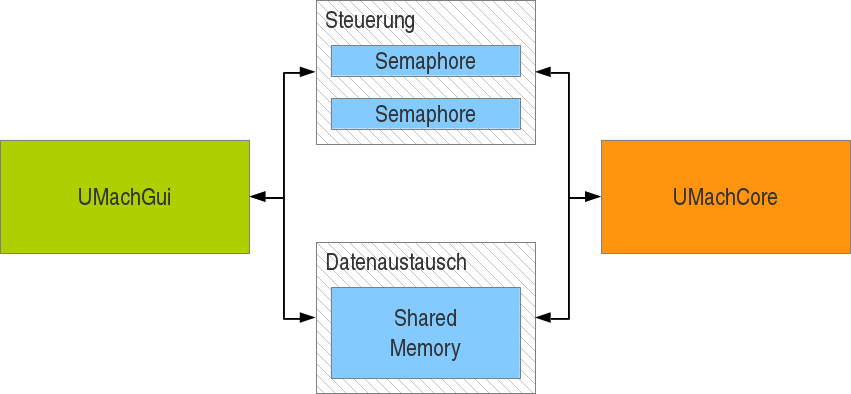
\includegraphics[width=\textwidth]{g1}
\end{frame}

\subsection{QSystemSemaphore}

\begin{frame}{\insertsubsection}
    \begin{itemize}
         \item Ressourcenzähler
         \item Blockiert Prozess wenn keine Ressource verfügbar
         \item Zugriff über ID
         \item aquire()\\
         Ressource anfordern
         \item release()\\
         Ressource freigeben
    \end{itemize}
\end{frame}

\subsection{QSharedMemory}

\begin{frame}{\insertsubsection}
    \begin{itemize}
         \item Prozessübergreifender Speicher
         \item Erster Konstruktoraufruf erzeugt Shared Memory
         \item Zugriff über ID
         \item attach()\\
         Anhängen an den Prozess
         \item detach()\\
         Abhängen vom Prozess
         \item Letzter Aufruf von detach() zerstört QSharedMemory
         \item Sicherstellung der Freigabe
    \end{itemize}
\end{frame}

\subsection{Kontrollzyklus}
\begin{frame}{\insertsubsection}
    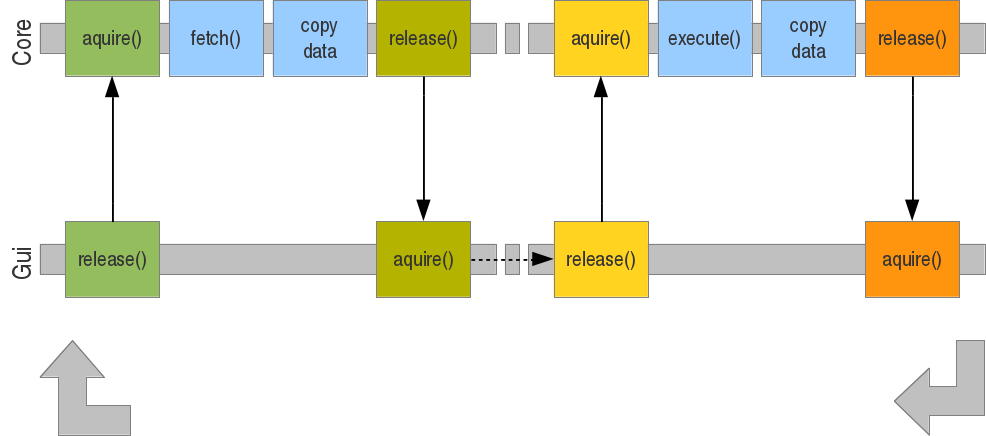
\includegraphics[width=\textwidth]{g2}
\end{frame}

\section{QT Bibliothek}

\subsection{Warum QT?}

\begin{frame}{\insertsubsection}
    \begin{itemize}
         \item Einfach zu verwenden, gute Dokumentation
         \item Plattformunabhängigkeit
         \item Flache Hierarchie - Einfach zu erweitern
         \item Vorhandene Erfahrungswerte
    \end{itemize}
\end{frame}

\subsection{Nachteile von QT}

\begin{frame}{\insertsubsection}
    \begin{itemize}
         \item Große Bibliothek\\
         für kleine Anwendungen ungeeignet
         \item Beispiel Digitaluhr\\
         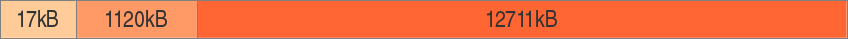
\includegraphics[scale=0.2]{g3}
         \item Großer Einrichtungsaufwand unter Windows (64 Bit)
    \end{itemize}
\end{frame}

\subsection{Signal \& Slot Prinzip}

\begin{frame}{\insertsubsection}
    \begin{itemize}
         \item Alternative zu Callback
         \item Einfache Syntax
         \item Minimal langsamer als Callback
         \item Benötigt Meta Object Compiler
    \end{itemize}
\end{frame}

\subsection{Signal}

\begin{frame}[fragile]{\insertsubsection}
	\lstinputlisting[language=C++]{./Debugger/c2_signal.cpp}
\end{frame}

\subsection{Emit}

\begin{frame}[fragile]{\insertsubsection}
	\lstinputlisting[language=C++]{./Debugger/c2_emit.cpp}
\end{frame}

\subsection{Slot}

\begin{frame}[fragile]{\insertsubsection}
	\lstinputlisting[language=C++]{./Debugger/c2_slot.cpp}
\end{frame}

\subsection{Connect}

\begin{frame}[fragile]{\insertsubsection}
	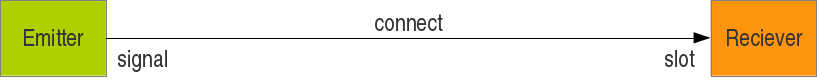
\includegraphics[width=\textwidth]{g4}
	\lstinputlisting[language=C++]{./Debugger/c2_connect.cpp}
	\lstinputlisting[language=C++]{./Debugger/c1.cpp}
\end{frame}

\section{GUI \& Demo}

\subsection{Projektdatei}

\begin{frame}{\insertsubsection}
    \begin{itemize}
         \item Projektdateu .umproject
         \begin{itemize}
         	\item Zugehörige Assemblerdateien
			\item Speicherung von Einstellungen und Haltepunkten
    	 \end{itemize}
         \item Benötigt Make-Routine
    \end{itemize}
\end{frame}

\subsection{Demo}

\begin{frame}{\insertsubsection}
    \begin{itemize}
    \item fibonacci.umx
    \item Haltepunkte
    \item Nächste Instruktion
    \item Registerinhalt
    \end{itemize}
\end{frame}

\subsection{Ausblick}

\begin{frame}{\insertsubsection}
    \begin{itemize}
    \item Speichern von Optionen
    \item Symbolinformation
    \item Manipulation Daten \& Zustand
    \item Weitere Ideen
    \begin{itemize}
    	\item Speicheranzeige
    	\item Graphische Darstellung Speicherbelegung
    	\item ...
    \end{itemize}
    \end{itemize}
\end{frame}

\part{Demos}
\section{Demo-Programme}
\begin{flushright}
Willi Fink
\end{flushright}





\end{document}
